% app2.tex (file to switch to appendix mode)

\chapter[\bassPiece]{}

\vspace*{3cm}
\begin{center}
\textsc{for solo contrabass}

\vspace*{3.5cm}

\HRule{0.5pt}


\LARGE \textbf{\uppercase{\bassPiece}}
\HRule{2pt}

\vspace{1.3cm}

\normalsize October, 2019
\date{}

\vspace*{5\baselineskip}

Rhys Gray

\end{center}
\newpage
\newpage

\section*{Program Notes}
Inspired by the eponymous short story by Ray Bradbury, \bassPiece\space is a composition for solo contrabass, and uses \hyperref[sec:subharmonics]{subharmonics} and \hyperref[sec:multiphonics]{multiphonics}. 
Similarly like the namesake, this world is filled with danger but also beauty. 
It is non-programmatic, and my intent with Veldt was to create a soundworld and space that the performer was able to `roam around' in, and features several sections of improvisation on pitch-sets.

\subsubsection*{Subharmonics}
To play subharmonics, one should place the bow at the 6th partial of the harmonic series of the fingered pitch, and bow with excessive pressure and an absolutely consistent speed. 
The increased pressure will distort the vibration of the string, producing a phase loop which, in turn, produces the subharmonic. 
Subharmonics are achieved through precise control of torsional oscillation, which usually produces the sound of an amateur string player's heavy handed, slow bowing. 
The production of subharmonics can be aided by using older strings (which work better due to fats building up on the strings). 
Making a counter-clockwise half-twist in the string can also make it easier to produce octave and major second subharmonics (additional twists can help achieve lower subharmonics, at the expense of higher ones).

\subsubsection*{Multiphonics}
Multiphonics are achieved through clusters of close harmonic nodes, and by playing a harmonic close to the highest partial.
  Note that not all of these pitches will actually sound in practice.
  
  Multiphonics are notated as a harmonic position using a diamond notehead, with an `M' above the note to be fingered.
  Where the string used is ambiguous, it is notated below the sounding pitch as a small, bracketed notehead.
  Precise tuning is given in cents, and unless otherwise notated, is intended for the first note that the multiphonic is attached to.\footnote{100 cents is equal to a semitone. Therefore, +51c is roughly equal to half a semitone sharp. Cents have been used due to their precision compared to more granular accidentals such as the quartertone sharp.}
  The theoretical sounding pitches are given in a bracketed staff above the main stave.
  % Above the sounding pitches, the sounding partials are given (i.e. M IV [4th + 13th + 9th + 15th + 5th]).

  The bow should exert slightly more pressure than usual and should be drawn with a consistent speed which should be slower than for harmonics.
  The location of the bow can encourage or discourage upper or lower partials, and experimentation should be done during the practice of this work to achieve the pitches desired.

\section*{Notation}
\begin{itemize}

    \item Subharmonics are notated in the score using a square notehead for the fingering, with a small notehead at the desired resultant pitch. Where additional clarification is needed, `sh' is placed above.
    \begin{itemize}
      \item They are notated at pitch in the cue sized stave above, with a harmonic circle above them.
    \end{itemize}
    \item Multiphonics are denoted with a diamond notehead, marked with an M (see \autoref{fig:multiphonicsBassExample} for an example). 
    \begin{itemize}
      \item Precise tuning in cents (i.e. +41c) is provided to help the performer pitch the fingering required for the multiphonic to be produced.
      \item The multiphonic resultant pitches are notated at pitch in the cue sized stave above, with the cents tuning of the resultant pitches to the left or right of the notes.
    \end{itemize}
    \item Arrows denote gradual transitions to the technique that the arrow is pointing to.\begin{itemize}
      \item Arrows between notes denote transitions between the types of notes (i.e.\ \emph{normale} to harmonic finger pressure.)
    \end{itemize}
    \item Sounding pitch is provided in the ossia stave above.
    \item Bridge position is provided in the stave above, and denotes the vertical location of the bow. The bottom line is \emph{molto sul tasto} and the top line is \emph{molto sul ponticello}.
    \item For un-metered bars, approximate times are given above in seconds, and is linearly proportional (i.e.\ note spacing denotes approximate time.)
    \item Repeats are to be repeated for as long as instructed.
    % \item \emph{battuto} is letting the bow hit the string, with no horizontal movement.
    % \item \emph{gettato} is like battuto, but with a slight amount of horizontal movement.
    % \item \emph{jeté} is bouncing the bow on the string, letting gravity do the work in conjunction with horizontal movement.
    \item op denotes overpressure.
    \item sp denotes \emph{sul ponticello}.
    \item n denotes \emph{normale}.
    % \item msp denotes \emph{molto sul ponticello}.
    % \item similarly, st denotes \emph{sul tasto}, and mst denotes \emph{molto sul tasto}
\end{itemize}

\newpage\label{app:bassPiece Score}

% 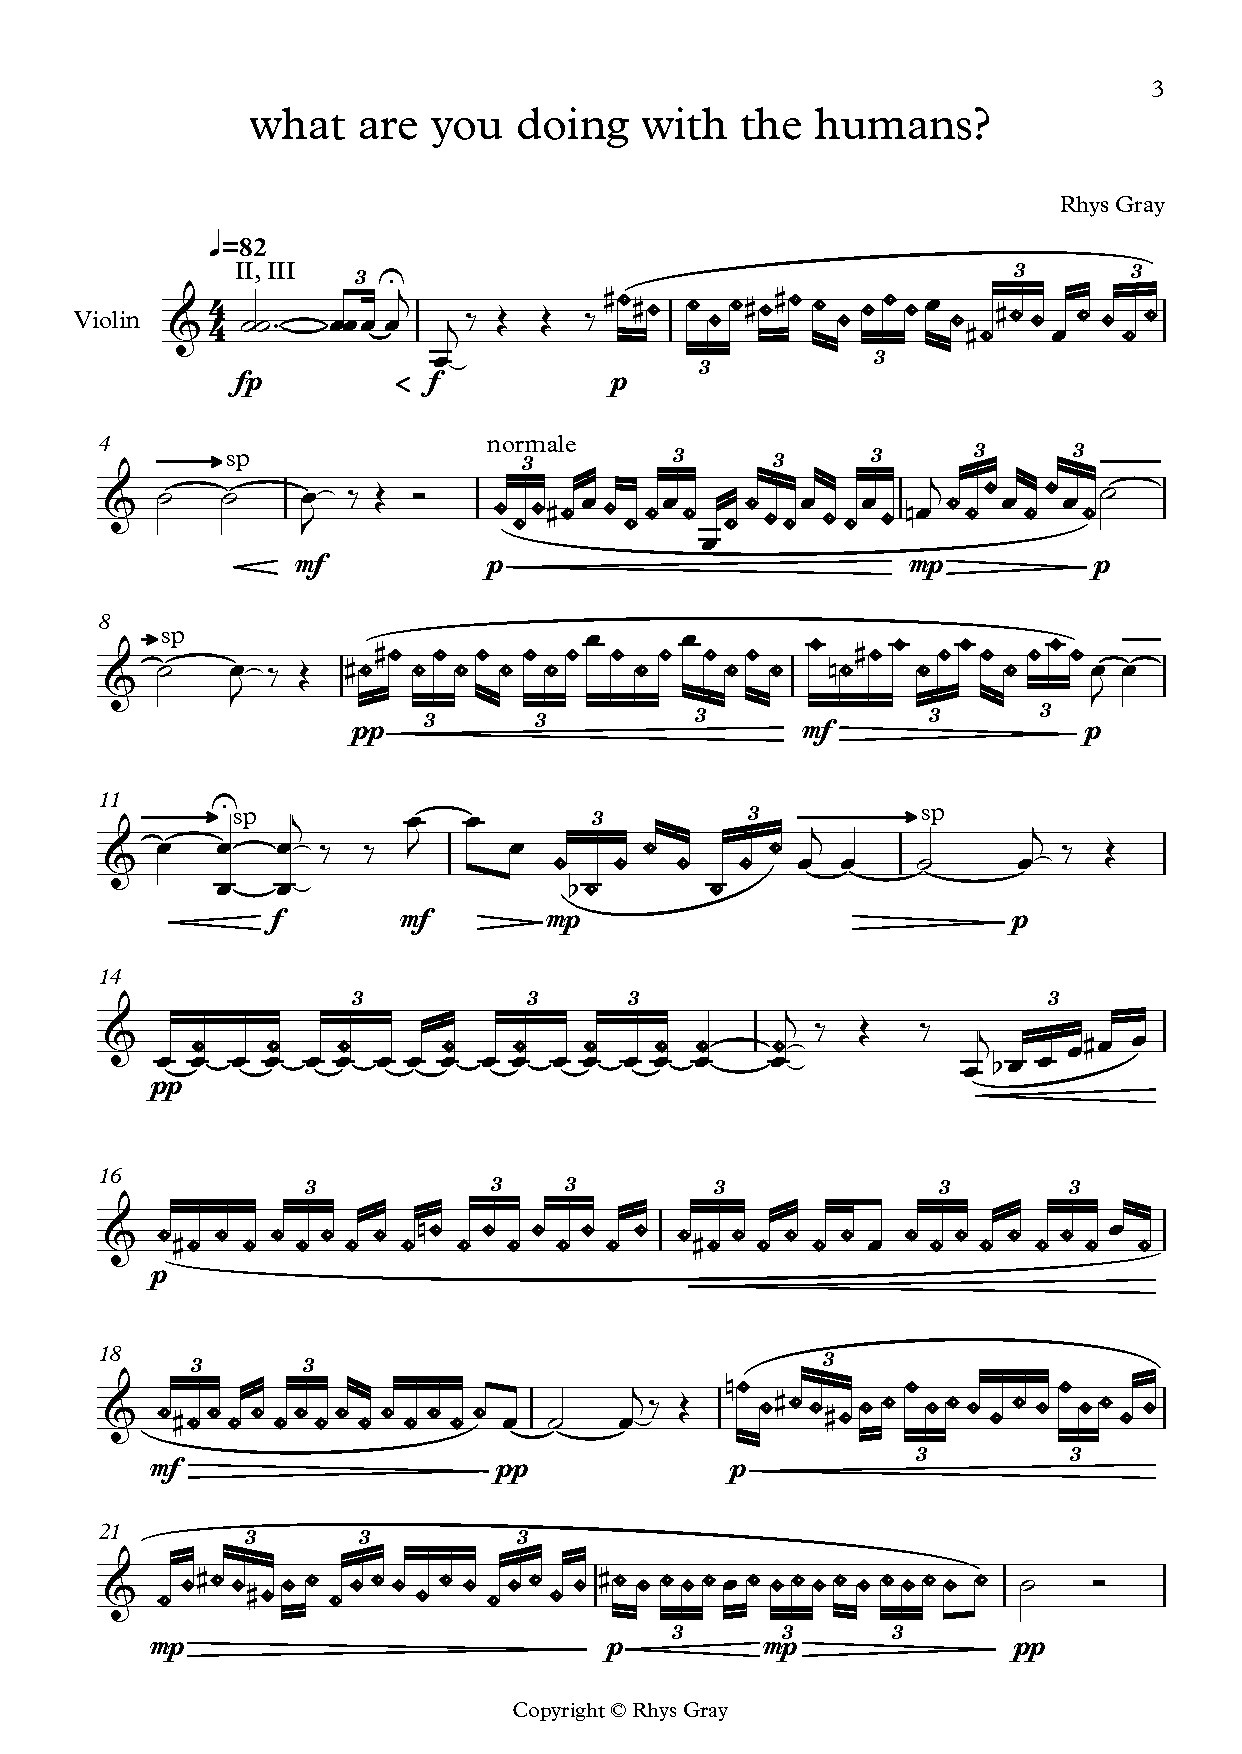
\includepdf[pages=-,pagecommand={},width=\textwidth]{resources/compositions/violin.pdf}

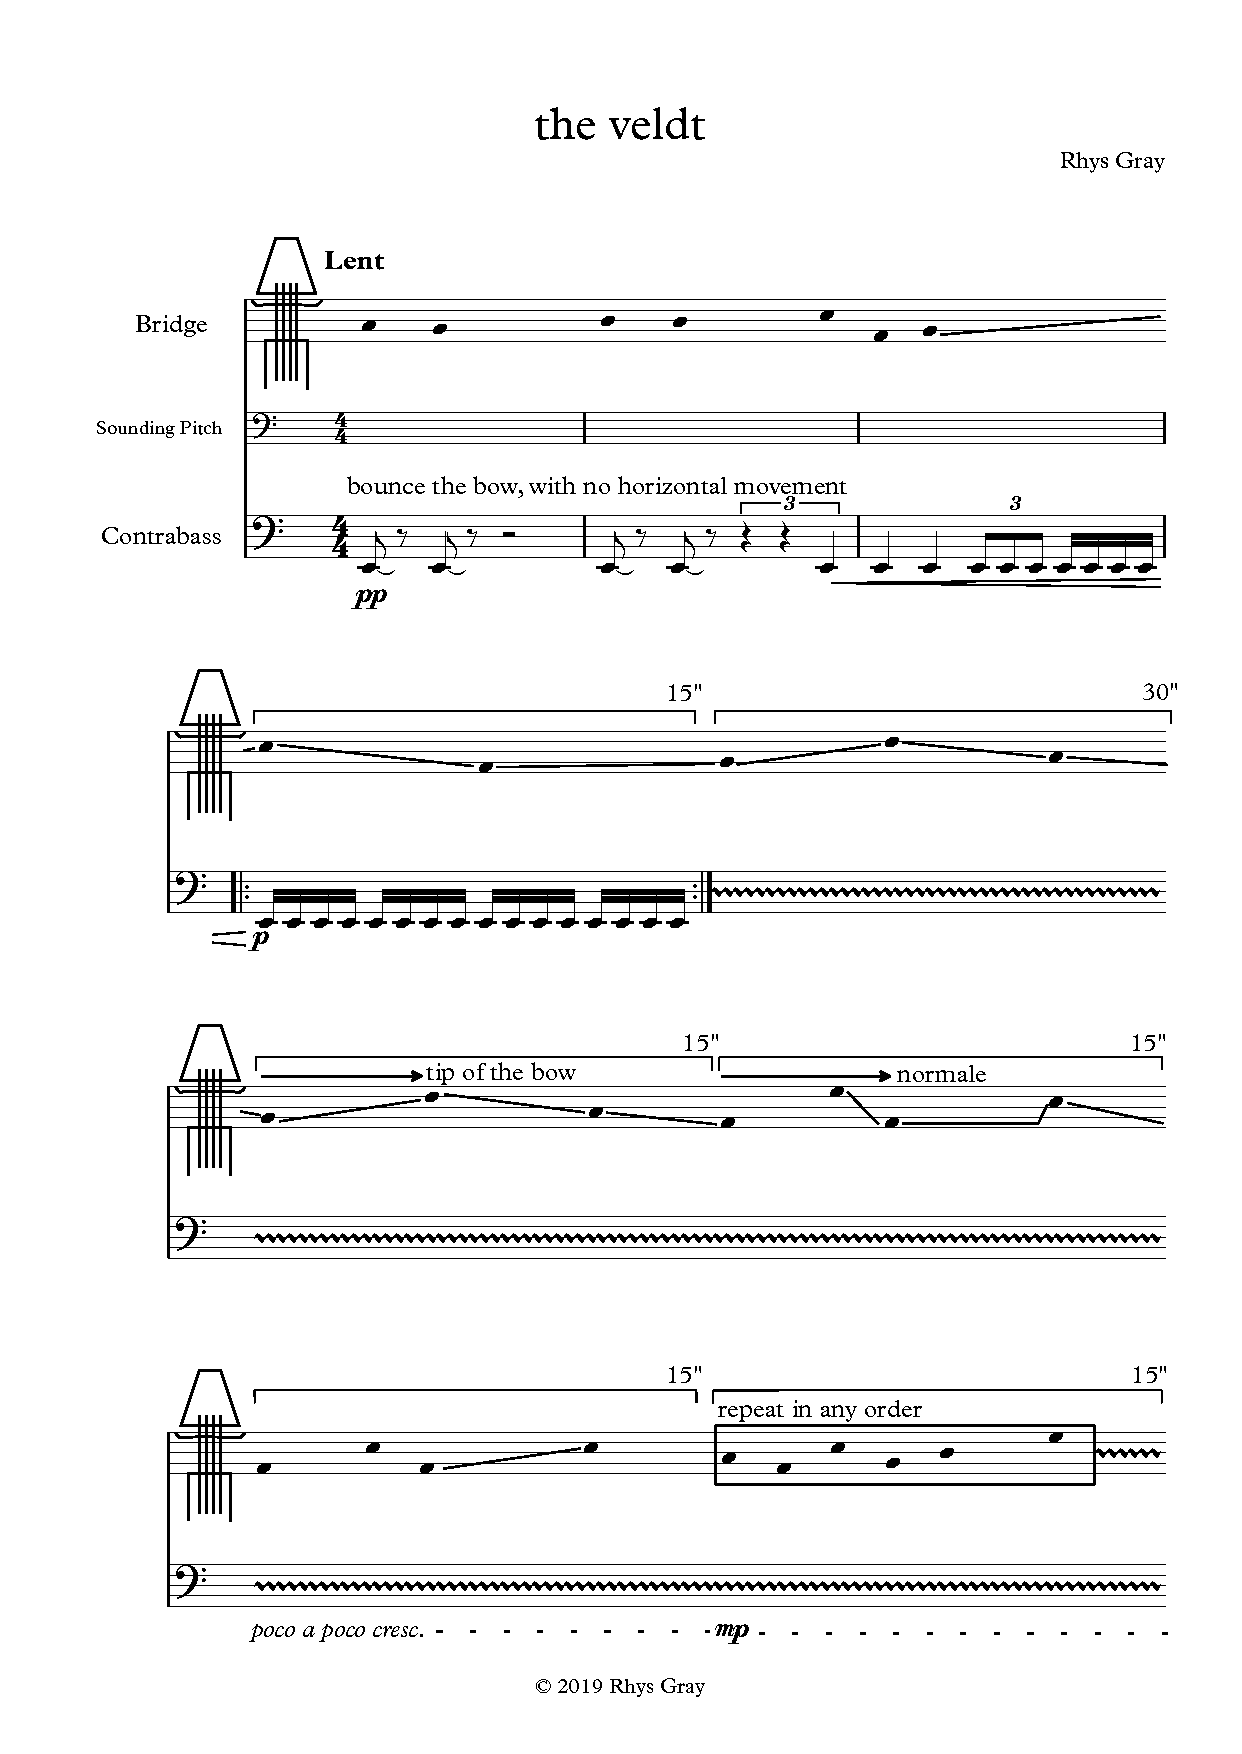
\includepdf[pages=-,pagecommand={}]{resources/compositions/bass.pdf}